\documentclass[12pt]{article}

\usepackage{dsfont}
\usepackage{amsmath}
\usepackage{graphicx}
\usepackage[margin=1in]{geometry}

\usepackage{bm}
\newcommand{\m}[1]{\mathbf{\bm{#1}}}
\newcommand{\R}{I\hspace{-4.4pt}R}

\setlength\parindent{0pt}

\begin{document}

Mickey Warner

\subsection*{Ozone in the Northeast United States}

The region we consider here comprises New England and a few states below along the east coast. This consists of 108 measurement locations (Figure 1). Measurements are made up of yearly ozone averages for 2015. An exploratory analysis showed a log transformation is suitable for a normal assumption. Though, the transformation may not be necessary, it at least better remedied some numerical issues.

\begin{figure}[ht]
\begin{center}
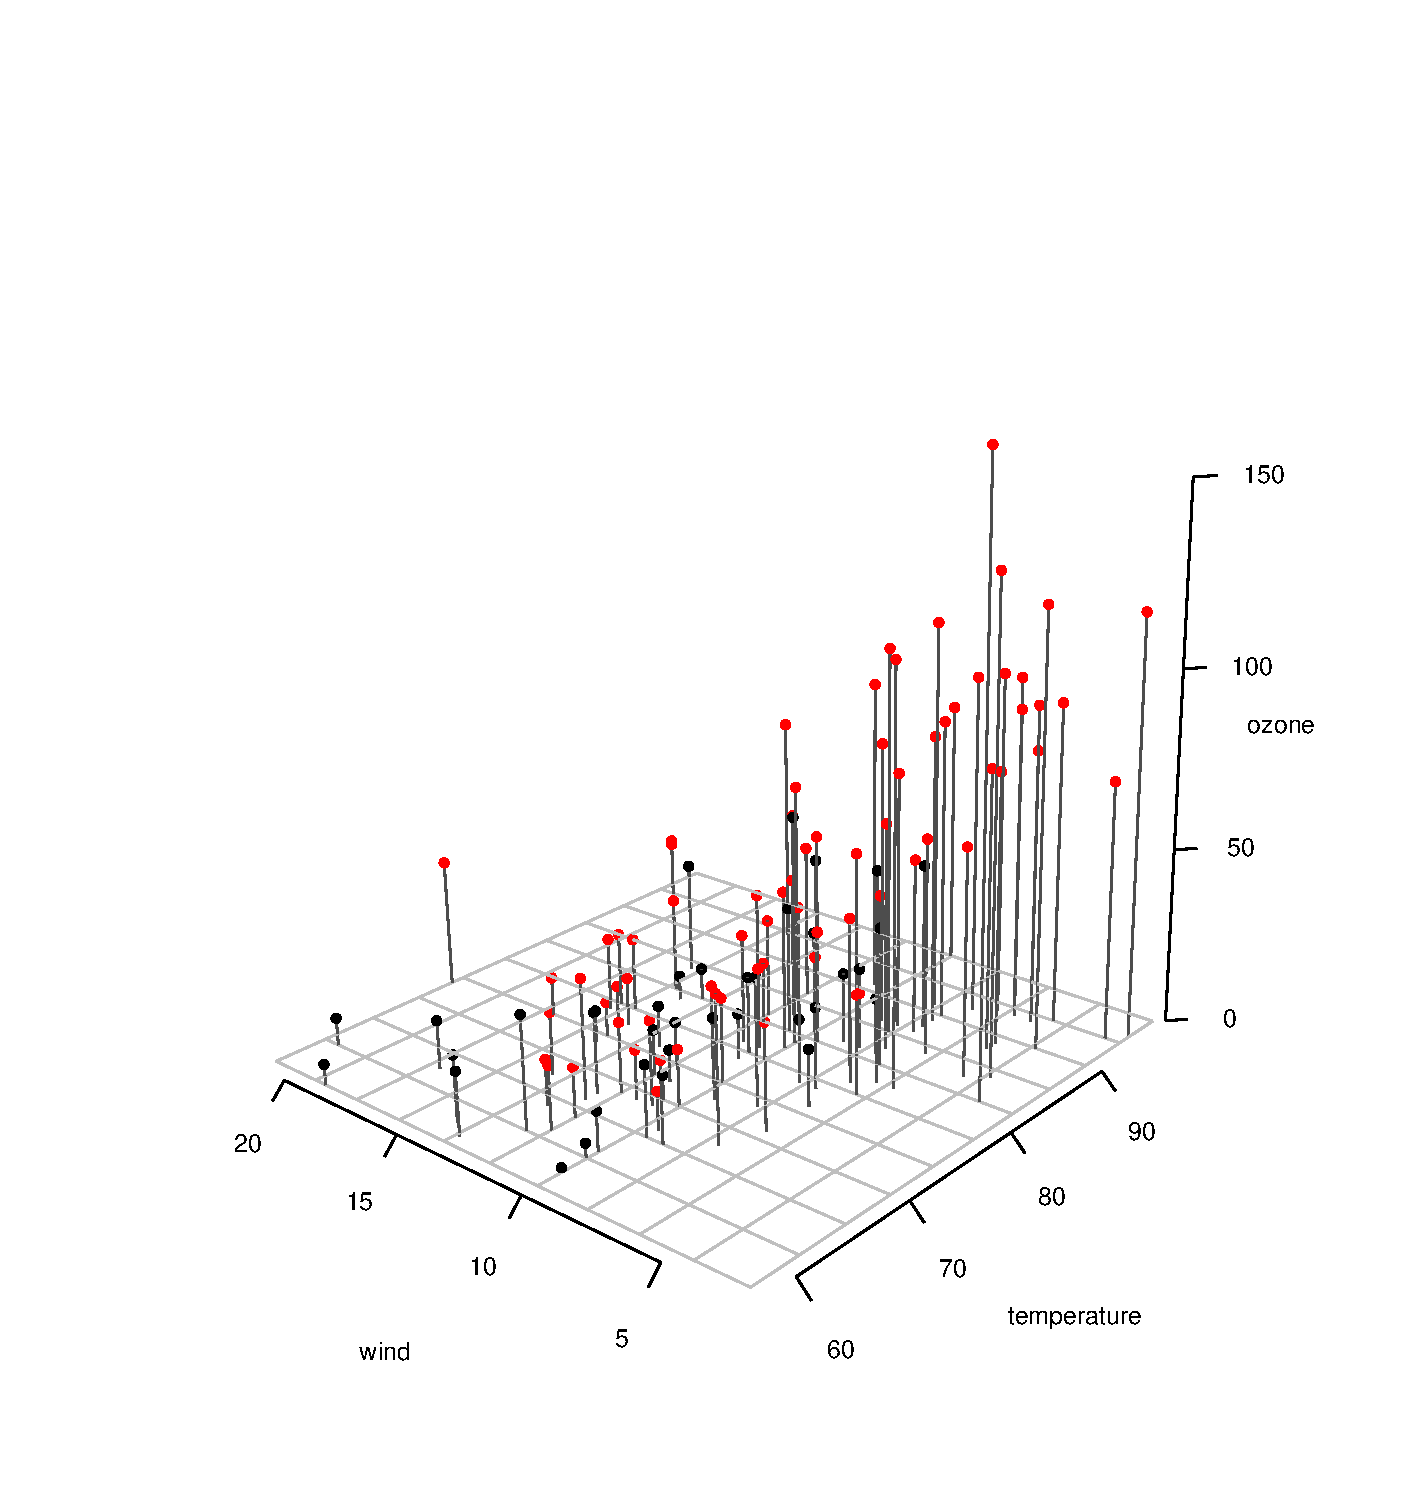
\includegraphics[scale=0.5]{figs/data.pdf}
\end{center}
\caption{Measurement locations of (log) ozone readings.}
\end{figure}

We explore possible trends in the data. Figure 2 hints at the possibility of some linear (or even quadratic) trends along some of the spatial dimensions, especially latitude. We fit a regression with lienar and quadratic terms in each direction. Covariates are selected with a step-wise procedure with AIC as its selection criterion.
\bigskip

We found that latitude had significant linear and quadratic trends, altitude had a linear trend, and there was evidence of interaction between latitude and altitude. There is some evidence of linear and quadratic trends in longitude.

\begin{figure}
\begin{center}
\includegraphics[scale=0.5]{figs/regression.pdf}
\end{center}
\caption{Each of three location types versus log ozone. The gray dots are the observed data, the black dots are the regression fit, and the liness represent the residuals.}
\end{figure}

\newpage

\subsection*{Variograms}

Using the residuals we compute a binned semivariogram from the data. We also look at the semivariogram in four directions to see if there is an anisotropy. The plots are given in Figure 3. We see from the right plot in Figure 3 that each direction produces more-or-less the same semivariogram, there is little difference between the curves. This suggests that we do not have enough evidence to believe there is anisotropy. Note altitude was treated as a covariate in generating these plots.

\begin{figure}[ht]
\begin{center}
\includegraphics[scale=0.5]{figs/variogram.pdf}
\end{center}
\caption{Omnidirectional semivariogram (left) and directional semivariograms (right).}
\end{figure}

We do a least squares fit to the omnidirectional semivariogram for parameters in the Mat{\'e}rn correlation. The function we are minimizing is
\[ f(u; \sigma^2,\phi,\kappa) = \sum_{i=1}^n\left[\sigma^2 (1 - \rho(u_i, \phi, \nu)) + \kappa\cdot 1_{(u>0)} - y_i\right]^2 \]
where $u_i$ is the distance obtain from the omnidirectional semivariogram, $y_i$ is the semivariance, $\kappa$ is the nugget, $\phi$ is the range, $\nu$ is the smoothness, $\rho$ is the Mat{\'e}rn correlation function, and $\sigma^2$ is related to the sill. We fix $\nu$ to be $0.5$, $1$, $1.5$, and $2.5$ and estimate the remaining parameters by maximizing $f$. The estimates for the parameters are shown in top left corners of the plots in Figure 4.

\begin{figure}[ht]
\begin{center}
\includegraphics[scale=0.5]{figs/matern.pdf}
\end{center}
\caption{LSE for the Mat{\'e}rn correlation.}
\end{figure}


\end{document}
